\documentclass[conference]{IEEEtran}
\IEEEoverridecommandlockouts

% ---------- packages ----------
\usepackage{cite}
\usepackage{amsmath,amssymb,amsfonts}
\usepackage{graphicx}
\usepackage{booktabs}
\usepackage{array}
\usepackage{xcolor}
\usepackage{url}
\usepackage{tikz}
\usetikzlibrary{arrows.meta,positioning,shapes.geometric,calc,fit,backgrounds}
\usepackage[hidelinks]{hyperref}

% ---------- tikz styles ----------
\tikzset{
  box/.style={rectangle, rounded corners=2pt, draw=black!70, fill=blue!6,
    align=center, minimum height=8mm, inner sep=4pt, font=\footnotesize},
  db/.style={cylinder, shape border rotate=90, aspect=0.25, draw=black!70,
    fill=orange!12, align=center, minimum height=10mm, font=\footnotesize},
  llm/.style={rectangle, rounded corners=2pt, draw=black!70, fill=green!8,
    align=center, minimum height=8mm, inner sep=4pt, font=\footnotesize},
  flow/.style={-{Stealth[length=2mm]}, draw=black!70},
  step/.style={rectangle, rounded corners=2pt, draw=black!70, fill=gray!8,
    align=center, minimum height=7mm, text width=20mm, inner sep=3pt, font=\scriptsize}
}

\begin{document}

\title{HospitAI: A Hospital Analytics Platform\\ Combining Patient Clustering, Clinical Sequence Mining\\ and AI-Generated Interpretation}

\author{\IEEEauthorblockN{Author Name}
\IEEEauthorblockA{\textit{Faculty of Computer Science} \\
\textit{University Name}\\
City, Country \\
author@email.example}}

\maketitle

\begin{abstract}
Hospitals collect a lot of electronic health record (EHR) data, but most of it stays unused for understanding patient groups and their care over time. We present HospitAI, a web platform that brings together three analytics steps in one place. First, it groups patients with K-Prototypes, a clustering method that works with mixed numerical and categorical data. Second, it mines frequent clinical sequences with a pipeline built around PrefixSpan, adapted to the medical domain. Third, it uses a large language model (LLM) to turn the numerical output into short descriptions that both doctors and patients can read. Our main technical contribution is the sequence-mining pipeline. Instead of ranking patterns only by how often they appear, we score them with a geometric mean lift measure and apply several diversity filters, so the results favour clinically meaningful care paths over frequent but trivial ones. We also mine each patient cluster on its own, and we treat statistical outliers as a separate group, which lets rare but important pathways such as oncology, dialysis and heart failure become visible. On a synthetic dataset of about 22{,}000 patients we obtain four stable clusters and per-cluster pattern sets that match recognisable care populations.
\end{abstract}

\begin{IEEEkeywords}
hospital analytics, patient clustering, K-Prototypes, sequential pattern mining, PrefixSpan, large language models, electronic health records
\end{IEEEkeywords}

\section{Introduction}

Modern hospitals store huge amounts of data in electronic health record (EHR) systems. Every visit leaves a trace: diagnoses, prescribed drugs, procedures and care plans. In theory this data could help managers and doctors understand who their patients are and how care actually happens. In practice most of it is never analysed, because the tables are large, messy and hard to read without technical skills.

There are three problems that make this kind of analysis difficult. The first one is that patients are very different from each other. A young person with a single broken bone and an elderly patient with diabetes, high blood pressure and kidney failure do not belong in the same bucket, yet a simple average over all patients hides this variety. The second problem is that care is not a single snapshot. It is a sequence of events that unfolds over months or years, and the order of those events often carries the clinical meaning. The third problem is communication. Even when a model produces a good result, the output is usually a list of numbers or codes that a clinician or a patient cannot interpret quickly.

In this paper we describe HospitAI, a web platform that addresses these three problems together. The platform was developed as part of an undergraduate thesis. It connects a clustering step, a sequence-mining step and a language step, so the same patient data can be looked at from several angles in one tool.

For the first problem we use K-Prototypes \cite{huang1998kprototypes}, a clustering algorithm made for mixed data, because clinical features are partly numerical (age, number of medications) and partly categorical (gender, main care plan). For the second problem we build a sequence-mining pipeline on top of PrefixSpan \cite{pei2004prefixspan}, and we adapt it to clinical data so that it returns useful care paths instead of obvious repetitions. For the third problem we add a large language model (LLM) that reads the computed statistics and writes a short summary in plain language for two audiences, the medical staff and the patient.

The contributions of this work can be summarised as follows.

\begin{itemize}
  \item An integrated, working platform that combines mixed-data patient clustering, clinical sequence mining and AI-generated interpretation, with a clear separation between the offline analytics and the web application that serves the results.
  \item A feature-engineering process that turns several raw EHR tables into a compact set of numerical and categorical patient features, with explicit handling of skewed values, missing vitals and statistical outliers.
  \item A domain-adapted sequence-mining pipeline around PrefixSpan. We rank patterns with a geometric mean lift score and a set of diversity rules, which strongly reduces trivial output and keeps clinically meaningful care paths near the top.
  \item A practical use of an LLM as a controlled ``verbaliser'' over fixed statistics, plus a guarded natural-language-to-SQL agent, so non-technical users can both read and ask questions about the data.
\end{itemize}

The rest of the paper is organised as follows. Section~\ref{sec:related} reviews related work on care-pathway mining and patient clustering. Section~\ref{sec:system} gives the system overview. Section~\ref{sec:methods} explains the three analytics components. Section~\ref{sec:results} reports the main results, and Section~\ref{sec:conclusion} discusses limitations and future work.

\section{Related Work}
\label{sec:related}

The idea of learning patient groups and care paths from health data is not new, and our work builds on several lines of research.

\textbf{Surveys of patient-pathway analysis.} Two recent reviews give a good map of the field. Rosa et al. \cite{rosa2022modelling} survey how patient pathways are modelled and mined, and they separate sequence-mining approaches from process-mining approaches. Flothow et al. \cite{flothow2023} review the analytical methods used to find sequences of healthcare utilisation, and they note an interesting split: clustering is mostly used to describe full care trajectories, while pattern-mining methods are mostly used to find shorter subsequences. HospitAI sits exactly between these two groups, because we first cluster patients and then mine sequences inside each cluster.

\textbf{Combining clustering and sequence mining.} The work closest to ours mixes the two ideas. Najjar et al. \cite{najjar2018twostep} propose a two-step method that first clusters individual medical visits with K-Prototypes and then builds higher-level treatment pathways. This is a strong precedent, because it uses the same mixed-data clustering algorithm that we use. Baudrier et al. \cite{baudrier2022} combine a sequential pattern-mining algorithm with care-trajectory clustering on kidney cancer patients, and they show that the resulting groups differ in real outcomes such as mortality. Vogt et al. \cite{vogt2017} apply sequence clustering to ambulatory care pathways in insurance claims and find typical care patterns for heart-failure patients. Our design follows the same spirit, but we reverse the order: clustering comes first and defines the scope, then mining runs inside each scope.

\textbf{Sequence mining from EMR with interpretation.} Perer et al. \cite{perer2015mining} mine frequent event sequences from electronic medical records and link them to patient outcomes, with a strong focus on visual exploration. Their system shows that frequent sequences can recover care patterns that are clinically meaningful, and sometimes even unknown to the physician. This motivates our own attention to pattern quality, because raw frequency alone is not enough.

\textbf{Clustering of patients on EHR data.} Several papers study how to group patients well. Yang et al. \cite{yang2024} build a smart-healthcare system that clusters patients on mixed medical data, including text embeddings, and compare several clustering methods. Aljohani \cite{aljohani2024} compares eight clustering algorithms for patient stratification on EHR data and uses a multi-criteria framework to rank them. These works confirm that clustering is a useful tool for patient stratification, and that the choice of algorithm and evaluation metric matters a lot.

\textbf{Process mining as an alternative.} A different family of methods discovers care processes from event logs. Murazzano et al. \cite{murazzano2026} apply process mining to chronic respiratory patients and find high variability in their clinical pathways. We mention this line of work because it targets the same goal as our sequence mining, namely understanding how care really happens, but with a different technique.

In short, clustering and sequence mining are both well studied in healthcare, and a few works already combine them. What is still missing is a single, practical tool that connects cluster-scoped mining, a pattern ranking made for clinical usefulness, and an automatic interpretation layer that non-experts can read. HospitAI is our attempt to fill that gap.

\section{System Overview}
\label{sec:system}

\subsection{Architecture}

HospitAI is split into a web application and an offline analytics part. The web side has a frontend built with Next.js and a backend built with FastAPI. The backend follows a layered structure with no shortcuts between layers: the API routers call a service layer, the service layer calls a repository layer, and the repository layer talks to the database. All persistent data lives in a single PostgreSQL database. Figure~\ref{fig:arch} shows the main pieces.

The two heavy machine-learning steps, clustering and sequence mining, do not run inside the web request. They are separate Python scripts that we run offline, because they are slow and they only need to run when the data changes. Each script reads from the database, computes its result and writes it back into dedicated tables. The web application then only reads these tables, which keeps the user interface fast. A single large language model, accessed through the OpenAI API, is used for every text-generation task in the system.

\begin{figure}[t]
\centering
\begin{tikzpicture}[node distance=5mm and 7mm]
  \node[box, fill=blue!8] (fe) {Frontend\\(Next.js + Redux)};
  \node[box, below=of fe] (api) {Backend API\\(FastAPI routers)};
  \node[box, below=of api] (svc) {Service layer};
  \node[box, below=of svc] (repo) {Repository layer};
  \node[db, below=8mm of repo] (db) {PostgreSQL};
  \node[step, right=14mm of svc, text width=22mm] (ml) {Offline ML scripts:\\K-Prototypes\\PrefixSpan};
  \node[llm, left=12mm of svc, text width=18mm] (llm) {LLM\\(OpenAI GPT)};

  \draw[flow] (fe) -- (api);
  \draw[flow] (api) -- (svc);
  \draw[flow] (svc) -- (repo);
  \draw[flow] (repo) -- (db);
  \draw[flow] (svc) -- (llm);
  \draw[{Stealth[length=2mm]}-{Stealth[length=2mm]}, draw=black!70] (ml) |- (db)
       node[pos=0.28,right,font=\scriptsize]{read / write};
\end{tikzpicture}
\caption{High-level architecture. The web application reads precomputed results; the clustering and mining scripts run offline and persist their output into the database.}
\label{fig:arch}
\end{figure}

\subsection{Data}

For development and experiments we use a synthetic dataset generated with Synthea, an open-source patient generator. Synthetic data is a good choice for a student project because it avoids privacy and legal issues while keeping a realistic structure. The dataset contains about 22{,}284 patients and the usual clinical tables: encounters, conditions, medications, procedures, observations and care plans. A loading script reduces the data to a single hospital and a fixed set of providers, cleans the dates and computes a few helper fields such as patient age and treatment duration.

The same database stores both the raw clinical tables and the analytics output. Clustering writes one row per patient with the cluster label and a cached set of features. Sequence mining writes the discovered patterns and a link table that records which patient contains which pattern. The interpretation step stores the generated text in JSON columns next to the cluster and pattern rows, so a summary is computed only once and then reused.

\section{Methods}
\label{sec:methods}

This section describes the three analytics components: patient clustering, clinical sequence mining and AI interpretation.

\subsection{Feature Engineering and Clustering}

Clustering needs a clean table where each row is a patient and each column is a feature. Building this table is most of the work, because the raw EHR data is spread over seven tables and is not ready for a model. We compute the features with SQL aggregation queries and then join them on the patient identifier.

We build a large set of candidate features and later keep a smaller subset. The features are of two kinds. Numerical features include age, the number of active conditions, the total number of medications and procedures, and a ratio that compares preventive visits to reactive ones. Categorical features include gender, a pregnancy-history flag, several disease flags (diabetes, hypertension, heart disease), a binned condition burden, a body-mass-index category and the most important care plan of the patient.

A few choices are worth noting. Some counts are strongly skewed, so we apply a logarithmic transform before scaling. Numerical features are scaled to the same range with min-max scaling. Vital signs such as blood pressure are often missing, so instead of filling them with the mean we put them into bins and add an explicit ``Unknown'' bin, which keeps the information that a value was not measured. We do not one-hot encode the categorical features, because K-Prototypes handles them directly.

K-Prototypes \cite{huang1998kprototypes} extends K-Means to mixed data. It measures distance on numerical features with the usual squared Euclidean distance, and distance on categorical features by counting mismatches. The two parts are combined with a weight $\gamma$ that controls how much the categorical side matters. We use the Huang initialisation and let the library pick $\gamma$ automatically in the final run.

Before fitting, we remove statistical outliers with a z-score rule, but we do not throw them away. Outliers receive the special cluster label $-1$ and are stored like every other patient. This matters later, because these patients carry the high-acuity signal (cancer, dialysis, heart failure) that a balanced clustering tends to push aside. We choose the number of clusters with an elbow plot on the clustering cost, and we confirm the choice with a silhouette score computed on a mixed-data (Gower) distance, since the standard silhouette assumes a purely numerical space.

\subsection{Clinical Sequence Mining}

The second component looks at the order of clinical events. We define one sequence per patient, which is the patient's timeline of events sorted by date. Each event gets a type prefix so that its source table is always clear: \texttt{C} for a condition, \texttt{M} for a medication, \texttt{P} for a procedure and \texttt{CP} for a care plan. When several events happen on the same day we order them in a fixed clinical order (condition, then medication, then procedure, then care plan), so that the runs are reproducible.

Before mining we clean each timeline. We keep only the last two years of events per patient, we drop a small list of purely administrative items, we collapse immediate repetitions of the same item and we cap the timeline length, which keeps the search fast. The mining itself uses PrefixSpan \cite{pei2004prefixspan}, a classic algorithm that grows frequent patterns by projecting the database on each found prefix. We ask it for closed patterns with a length between three and six and a minimum support of one percent of the patients.

\begin{figure}[t]
\centering
\begin{tikzpicture}[node distance=3.2mm]
  \node[step] (a) {Raw events\\(C, M, P, CP)};
  \node[step, below=of a] (b) {Per-patient\\timelines};
  \node[step, below=of b] (c) {PrefixSpan\\(closed, len 3 to 6)};
  \node[step, below=of c] (d) {GML scoring\\+ type bonus};
  \node[step, below=of d] (e) {Diversity\\filters};
  \node[step, below=of e] (f) {Top patterns\\per scope};
  \foreach \x/\y in {a/b,b/c,c/d,d/e,e/f} \draw[flow] (\x) -- (\y);
\end{tikzpicture}
\caption{The sequence-mining pipeline. PrefixSpan is the engine, but the scoring and the diversity filters around it decide what the user finally sees.}
\label{fig:pipeline}
\end{figure}

The interesting part is what happens around PrefixSpan, shown in Figure~\ref{fig:pipeline}. If we rank patterns only by support, the top of the list is full of frequent but useless chains, for example routine dental cleaning steps that almost every patient receives. To fix this we rank patterns with a geometric mean lift (GML) score. For a pattern $p$ made of $k$ items with support $s(p)$ over $n$ patients, and with item supports $s(i)$, the score is
\begin{equation}
\mathrm{GML}(p) \;=\; \frac{s(p)/n}{\left(\prod_{i \in p} s(i)/n \right)^{1/k}} .
\end{equation}
This is the lift idea extended from two items to $k$ items through a geometric mean, and we compute it in log space for numerical stability. A pattern scores high when its whole chain is more frequent than we would expect from its individual items, which is a sign that the steps really go together.

We add two more ideas. First, a type-diversity bonus multiplies the score by $(1 + 0.3\,(t-1))$, where $t$ is the number of event types in the pattern. This rewards a real care trajectory that mixes conditions, drugs and procedures over a pattern that just repeats three medications. Second, we apply a set of diversity filters before we accept a pattern: we drop patterns with three same-type events in a row, we remove near-duplicates with a Jaccard test on their item sets, and we cap how many patterns may share the same first or last item. We also keep a small reserved quota for full-spectrum patterns that contain all four event types, so these rare but complete care paths are never crowded out.

Finally, we run the whole pipeline once per scope. We mine the global cohort, and then we mine each cluster on its own, including the outlier group with label $-1$. Patterns that already appear in the global scope are removed from the cluster results, so each cluster only shows what makes it different.

\subsection{AI Interpretation}

The last component makes the output readable. We use a single LLM, but we use it in a controlled way. The model never computes statistics by itself. Instead, our code first computes everything (cluster averages, disease rates, cohort statistics for a pattern) and then passes these fixed numbers to the model, with clear instructions to only describe them. This ``verbaliser'' design keeps the text grounded in real values and lowers the risk of invented facts.

The platform generates three kinds of text. For each cluster it writes a short card with a title, a colour, a description and a recommendation. On demand it writes a longer analysis of a cluster or of a single mined pattern, returned as structured JSON with fields such as a clinical interpretation, a plain-language summary, risk signals and recommendations. These results are cached in the database, so the model is called only once per item.

The platform also includes a question-answering agent built with LangGraph. A user can type a question in natural language, and the agent turns it into a read-only SQL query. The agent first classifies the question, then generates a query, then validates it. Validation is strict: the query must be a single \texttt{SELECT}, dangerous keywords are blocked, and a second model pass checks that the query matches the question. Only then is the query run, and the rows are summarised back in natural language. A role-scoping rule can restrict a doctor to their own patients.

\section{Results}

\label{sec:results}

The effectiveness of the proposed approach is illustrated using the Synthea dataset, which is introduced in Section~\ref{sec:system}. Out of 22{,}284 patients, only 21{,}995 patients have been clustered, and all outliers have been retained in a different class labeled as $-1$.

\subsection{Clustering}

To discover the optimal configuration, we performed a huge benchmarking procedure on 629 configurations. Configuration means feature subset selection (we tried more than sixty feature subsets), cluster number $k$, scaler used, categorical weight $\gamma$, random state and outlier threshold. For benchmarking, we calculated a score based on three metrics. First of all, the metrics are min-max normalized individually within the scope of all 629 configurations, and the score is then their linear combination with weights that reflect our confidence in them ($0.5$ for Gower silhouette, $0.3$ for Calinski-Harabasz index and $0.2$ for Davies-Bouldin index, inverted because the higher the score the worse the partition is). We chose the best clinically interesting configuration per $k$ value (we tried four, five and six), and from these three configurations we tried once again to optimize the hyperparameters and feature subset used in order to choose the best local configuration.

\begin{table*}[t]

\caption{Representative clustering configuration for each cluster number (feature vector based on the corresponding version id). CH index and DB index are computed from the FAMD embedding in the mixed score framework. The highest value obtained for each criterion is marked in bold font. The selected cluster number is $k=4$ (v55).}

\label{tab:clusters}

\centering

\footnotesize

\begin{tabular}{@{}l c c l c r c@{}}

\toprule

Config & $k$ & Gower & Per-cluster Gower & DB & CH & Score \\

\midrule

v55 (final) & 4 & \textbf{0.350} & 0.42, 0.20, 0.32, 0.40 & \textbf{0.72} & \textbf{26813} & \textbf{0.82} \\

v40 & 5 & 0.324 & 0.28, 0.22, 0.31, 0.19, 0.48 & 0.87 & 22547 & 0.74 \\

v60 & 6 & 0.287 & 0.17, 0.13, 0.47, 0.21, 0.38, 0.27 & 0.95 & 22273 & 0.70 \\

\bottomrule

\end{tabular}

\end{table*}

Table~\ref{tab:clusters} reports a representative configuration for each $k$. The choice of $k$ is made to be 4, with feature combination v55. It scores best overall (0.82) among the clinically meaningful runs, and does so across all individual metrics: the largest Gower silhouette, the largest Calinski-Harabasz score, and the smallest Davies-Bouldin score. We still eliminate one family of runs, which scores even better on paper. It achieves a score of 0.87 by segregating patients according to gender, but since the separation is meaningless clinically, we exclude them. Among the four clusters in the optimal run, three get a Gower silhouette per cluster greater than 0.30, and only one gets close to 0.20, compared with the results of five and six clusters where one and two clusters respectively have values less than 0.20. Since clusters will be used for the scope of the sequence mining analysis, we prefer to have the smallest $k$ possible while still having all the clusters be cohesive. The important features are the number of active conditions and patient age numerically, and condition burden, gender, diabetes, and heart disease categorically.

Figure~\ref{fig:heatmap} shows the per-cluster means of the numeric variables represented as a heatmap. There is certainly a morbidity gradient. That is, cluster 0 represents young people with low morbidity, while the rest of the clusters contain a progressively greater number of conditions. By interpreting all four clusters in conjunction with the categorical features, we see four distinct patient profiles, which the AI platform automatically labels as: Younger Injury Care (young, low morbidity), Pregnancy Focused Adults (reproductive women), Older High Risk (hypertensive polypharmacy adults), and Kids and Well Visits (pediatric/acute patients).

\begin{figure}[t]

\centering

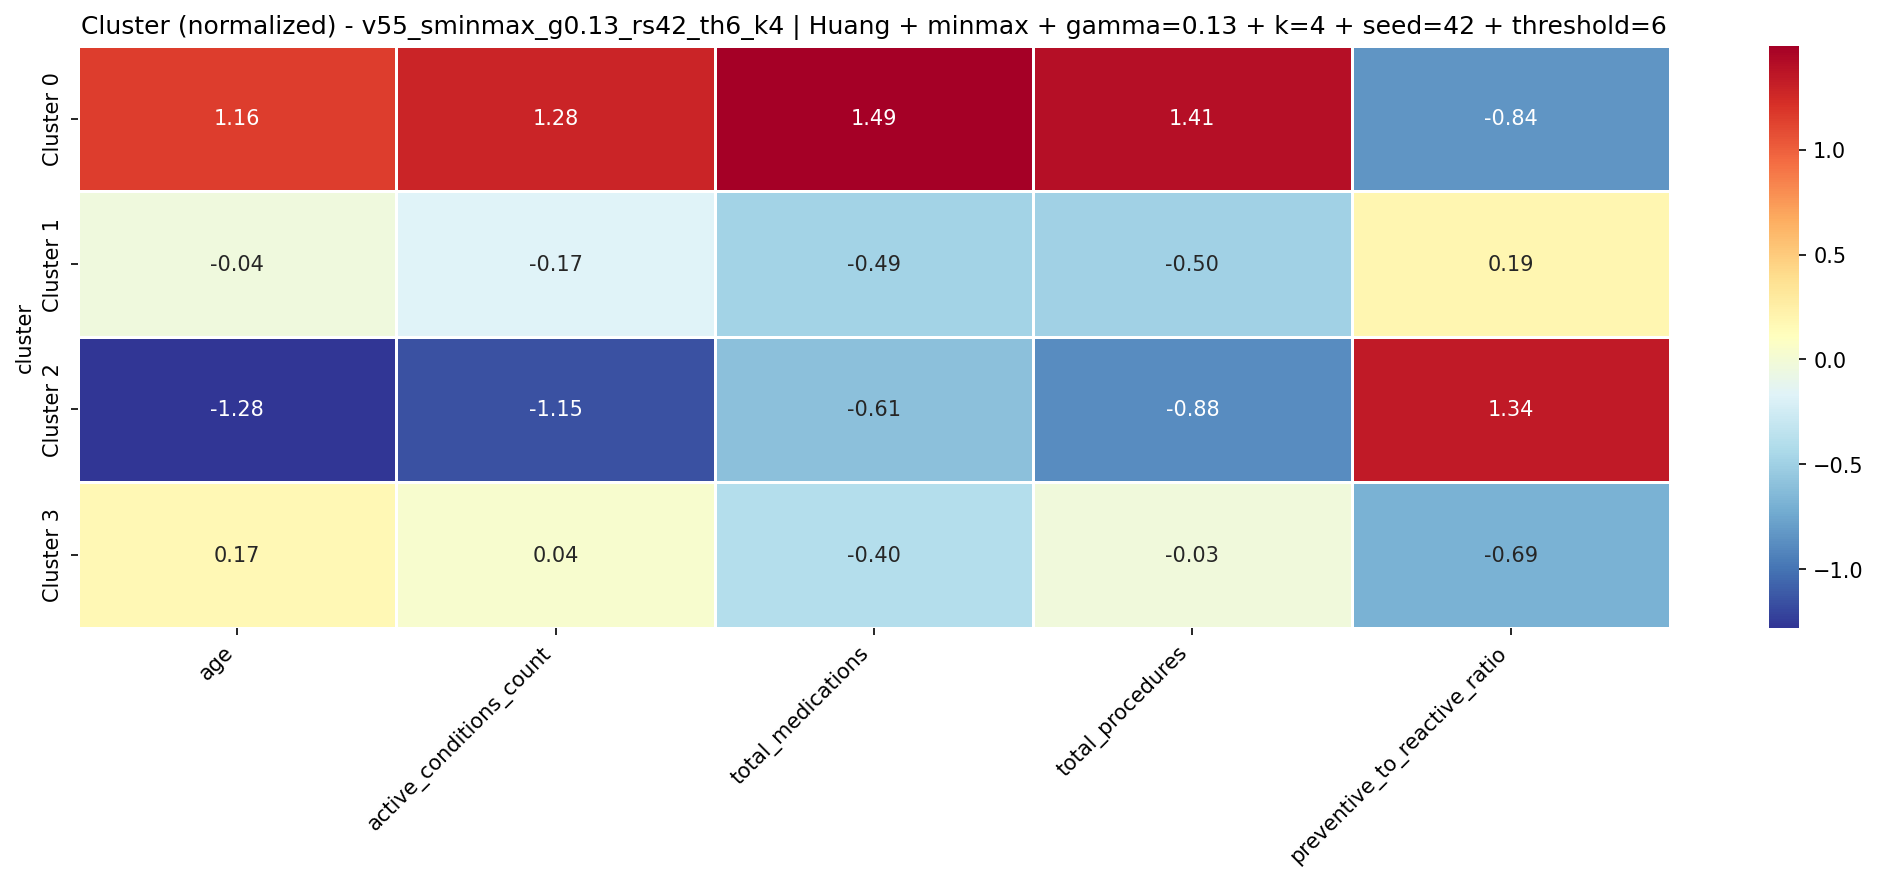
\includegraphics[width=0.95\linewidth]{figs/cluster_heatmap.png}

\caption{Z-scored numerical feature means per cluster ($k=4$). Warm colours are above the population average, cool colours below it.}

\label{fig:heatmap}

\end{figure}

\subsection{Sequence Mining}

The most straightforward demonstration of the impact of our pipeline can be seen through the transformation in the properties of the mined patterns as each new version is introduced. In Table~\ref{tab:ablation}, we present two sample patterns of at least four events from every one of these versions. The initial versions (v0-v2) rank patterns solely based on support, and therefore, the beginning of the ranking consists of common yet meaningless sequences, which consist mainly of similar dental cleanings that about 93\% of the patients undergo. With v3 and onwards, geometric mean lift-based ranking along with diversity filters were applied, and at the top of the ranking, clinically consistent care pathways can be seen. Version v4 also filters out consecutive occurrence of similar events, which is why the long sequence of procedure events related to a diabetic eye exam no longer appears from v4 onwards. At v6, when social status events are removed and reserved space for full spectrum patterns was set aside, diverse combinations of conditions, care plans, medicines and procedures appear despite their low support scores.

\begin{table}[t]

\caption{How the mined patterns evolve across miner versions}

\label{tab:ablation}

\centering

\scriptsize

\begin{tabular}{@{}l p{0.72\linewidth} r@{}}

\toprule

Ver. & Example pattern (length $\ge 4$) & Sup. \\

\midrule

v0 & dental consultation $\rightarrow$ dental care $\rightarrow$ supragingival scaling $\rightarrow$ subgingival scaling & 93\% \\

v0 & supragingival scaling $\rightarrow$ subgingival scaling $\rightarrow$ gingivae exam $\rightarrow$ oral health education & 93\% \\

\addlinespace

v1 & supragingival scaling $\rightarrow$ subgingival scaling $\rightarrow$ gingivae exam $\rightarrow$ oral health education & 63\% \\

v1 & dental care $\rightarrow$ supragingival scaling $\rightarrow$ subgingival scaling $\rightarrow$ oral health education & 63\% \\

\addlinespace

v2 & dental consultation $\rightarrow$ dental care $\rightarrow$ subgingival scaling $\rightarrow$ gingivae exam $\rightarrow$ oral health education & 62\% \\

v2 & dental referral $\rightarrow$ dental consultation $\rightarrow$ dental care $\rightarrow$ subgingival scaling $\rightarrow$ oral health education & 57\% \\

\midrule

v3 & tropicamide eye drops $\rightarrow$ gonioscopy $\rightarrow$ fundoscopy $\rightarrow$ diabetic eye exam & 3\% \\

v3 & furosemide $\rightarrow$ oxygen by mask $\rightarrow$ prone position $\rightarrow$ furosemide & 2\% \\

\addlinespace

v4 & acute bronchitis $\rightarrow$ respiratory therapy $\rightarrow$ respiratory function test $\rightarrow$ acetaminophen & 3\% \\

v4 & salmeterol-fluticasone inhaler $\rightarrow$ albuterol $\rightarrow$ spirometry $\rightarrow$ depression screening & 2\% \\

\addlinespace

v5 & subgingival scaling $\rightarrow$ gingivae exam $\rightarrow$ sodium fluoride gel $\rightarrow$ fluoride treatment & 35\% \\

v5 & dental bitewing X-ray $\rightarrow$ gingivae exam $\rightarrow$ sodium fluoride gel $\rightarrow$ fluoride treatment & 19\% \\

\addlinespace

v6 & acute bronchitis $\rightarrow$ respiratory therapy $\rightarrow$ respiratory function test $\rightarrow$ acetaminophen & 3\% \\

v6 & chest X-ray $\rightarrow$ furosemide $\rightarrow$ oxygen by mask $\rightarrow$ prone position $\rightarrow$ furosemide & 1\% \\

\bottomrule

\end{tabular}

\end{table}

Frequent pattern mining from each scope individually yields 175-252 frequent patterns per cluster. Examples of representative frequent patterns are listed in Table~\ref{tab:patterns}. Each cluster has a unique signal dominating its set of frequent patterns. For example, in Cluster~0, the dominant signal relates to acute care episodes. In Cluster~2, the chronic disease management includes antihypertensive drugs combined with screenings, or furosemide along with oxygen therapy to manage fluid overload. The most valuable benefit is obtained from the outlier scope. Since we mine each individual scope independently, high-cost combinations like chemotherapy and cisplatin leading to hospice care, or dialysis and epoetin, will dominate the results. Otherwise, these pathways fall under the global support threshold and would be missed when mining all cases at once.

\begin{table}[t]

\caption{Representative mined pathways by scope (ranked by GML).}

\label{tab:patterns}

\centering

\footnotesize

\begin{tabular}{@{}p{0.16\linewidth}p{0.74\linewidth}@{}}

\toprule

Scope & Pattern \\

\midrule

Cluster 0 & Fracture of bone $\rightarrow$ Fracture care $\rightarrow$ Bone immobilization \\

Cluster 1 & Normal pregnancy $\rightarrow$ Pregnancy test $\rightarrow$ Ultrasound for fetal viability \\

Cluster 2 & Furosemide $\rightarrow$ Oxygen by mask $\rightarrow$ Prone position $\rightarrow$ Furosemide \\

Cluster 3 & Acute allergic reaction $\rightarrow$ Epinephrine injection $\rightarrow$ Prednisone \\

Outliers ($-1$) & Chemotherapy + radiation $\rightarrow$ Cisplatin $\rightarrow$ Hospice care \\

\bottomrule

\end{tabular}

\end{table}

\subsection{AI Layer}

Upon running the K-Prototypes script, the AI creates a short card per cluster based on the statistics generated beforehand and determines the cluster title, its colour theme that will be used in all mentions of the cluster on the platform, its description, an insight and a recommendation for each. Figure~\ref{fig:platform_clusters} depicts how these cards look like in the dashboard. Since the model uses only the precomputed values, the card matches the heatmap and the prevalence rates by assigning high risk and a cardiology-related recommendation to the high-burden cluster, and a healthy, preventive profile otherwise.

\begin{figure}[t]

\centering

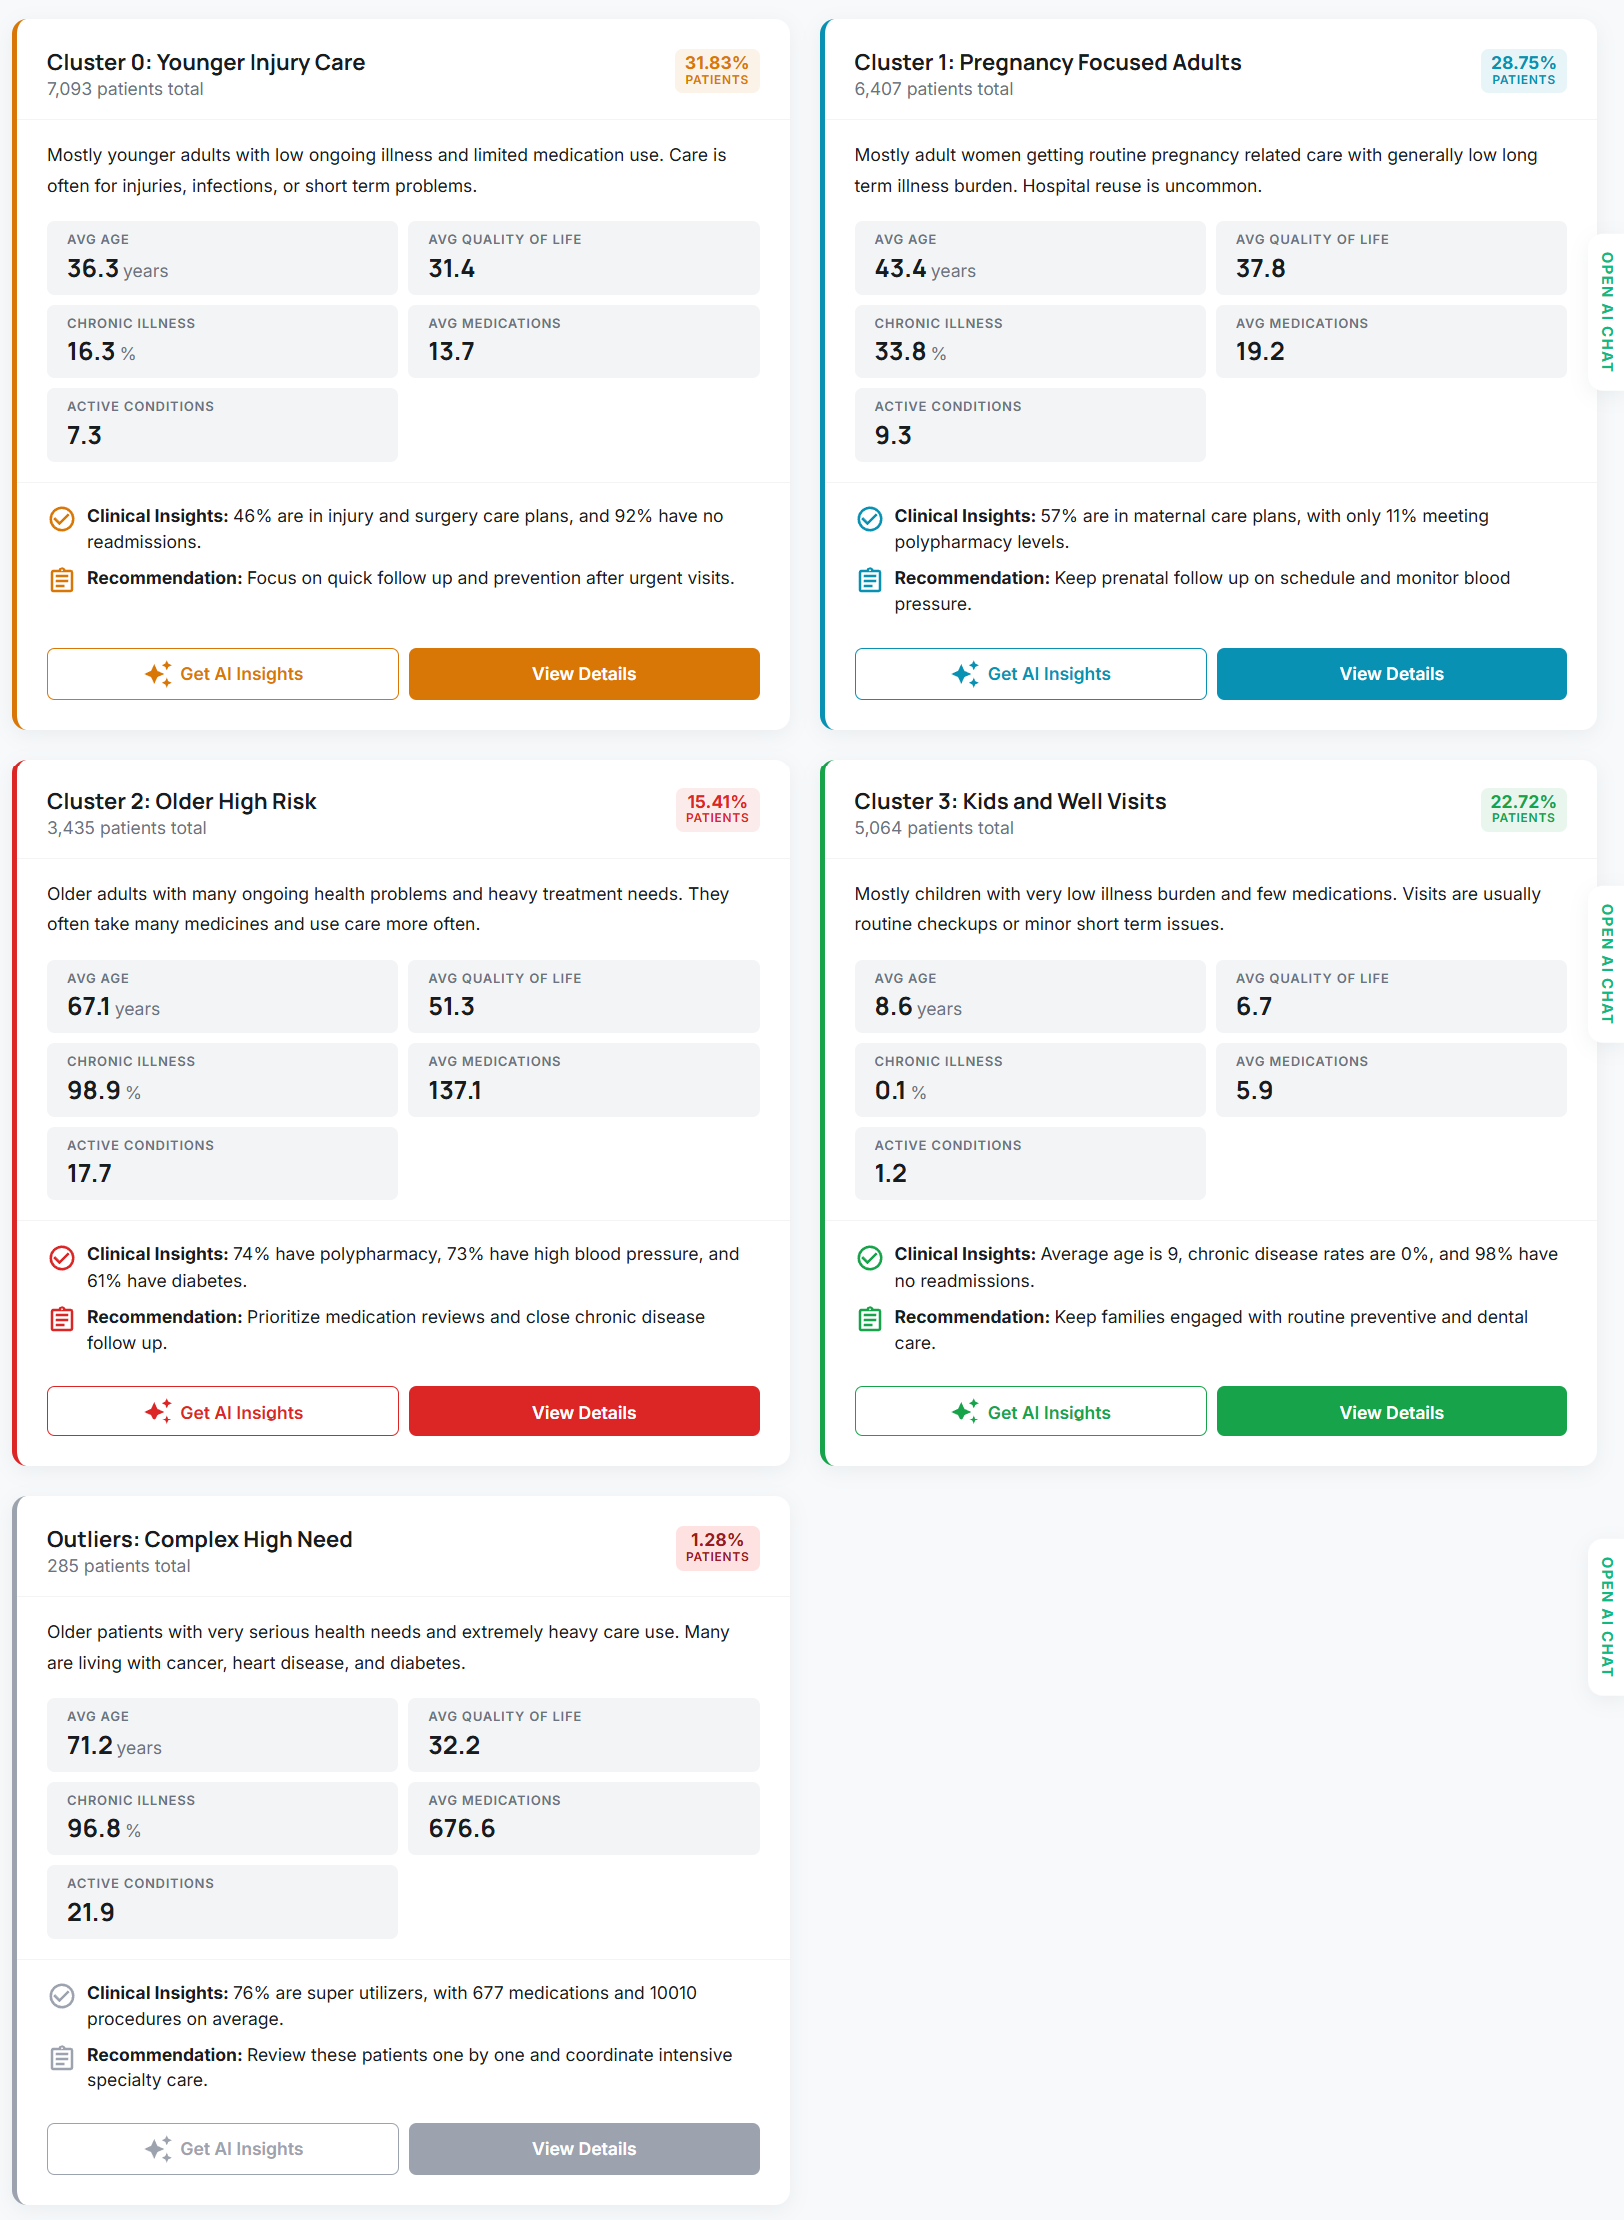
\includegraphics[width=\linewidth]{figs/platform_clusters.png}

\caption{The clusters as shown in the platform. The title, colour, description, insight and recommendation of each card are produced automatically by the AI when the clustering script runs.}

\label{fig:platform_clusters}

\end{figure}

Above and beyond the card information, the platform generates a more detailed report about every identified cluster or pattern using the mining algorithm, which has dual purposes to serve, one, as a clinical explanation intended for clinicians, and another, as a simpler, layman's summary for someone who lacks a medical perspective. This kind of explanation is depicted in Figure~\ref{fig:platform_interpretation}.

\begin{figure}[t]

\centering

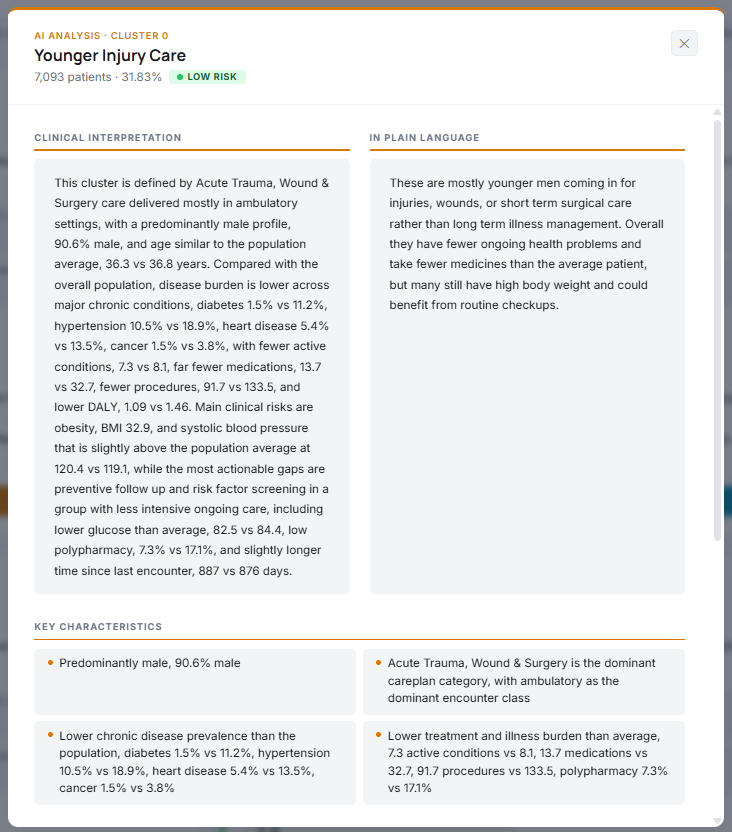
\includegraphics[width=\linewidth]{figs/platform_interpretation.png}

\caption{A cluster AI interpretation in the front end, written for both a clinician and a reader without medical training.}

\label{fig:platform_interpretation}

\end{figure}

Finally, the natural-language-to-SQL agent lets a user ask free questions. We tested it on questions of different difficulty, including non-trivial ones that need several joins. Table~\ref{tab:agent_example} lists two such questions: the first joins several clinical tables, the second joins the cluster and the sequence-mining tables. The answers are correct almost every time, and the guard layer blocked every attempt to run a non-\texttt{SELECT} statement. When the agent cannot build a valid query or finds no matching data, it plainly says it could not complete the task instead of inventing an answer.

\begin{table}[t]

\caption{Two example exchanges with the natural-language-to-SQL agent. The first needs several joins across the clinical tables, while the second joins the cluster and the sequence-mining tables.}

\label{tab:agent_example}

\centering

\footnotesize

\begin{tabular}{@{}p{0.48\linewidth}p{0.44\linewidth}@{}}

\toprule

Question & Agent answer \\

\midrule

How many distinct female patients over 60 with a diabetes diagnosis were also prescribed metformin and had at least one emergency encounter? & There were 144 distinct female patients over 60 with a diabetes diagnosis who were prescribed metformin and had at least one emergency encounter. \\[4pt]

Which mined care pathway is followed by the most patients in cluster~2, and how many of them follow it? & In cluster~2, the most common mined pathway is ``M:sodium fluoride 0.0272 MG/MG Oral Gel $\rightarrow$ P:Dental fluoride treatment $\rightarrow$ P:Oral health education'', followed by 1{,}265 patients. \\

\bottomrule

\end{tabular}

\end{table}

A full quantitative evaluation of the agent and of the generated summaries is left for future work, as discussed next.


\section{Discussion and Conclusion}
\label{sec:conclusion}

We presented HospitAI, a platform that joins three analytics steps over hospital data: mixed-data patient clustering, clinical sequence mining and AI-generated interpretation. The clustering gives a small number of readable patient groups. The sequence mining, with its geometric mean lift ranking and its diversity filters, returns care paths that are clinically meaningful instead of just frequent. The language layer turns the numbers into short summaries and lets users ask questions in plain English.

We see a few clear strengths. The cluster-then-mine design keeps each result local to a patient group, which makes the patterns easier to read. Treating outliers as their own scope is a simple idea that pays off, because it brings rare but important pathways back into view. The verbaliser design, where the model only describes precomputed numbers, is a practical way to use an LLM without letting it invent facts.

There are also honest limitations. The data is synthetic, so the patterns reflect how Synthea models care and not a real hospital. We did not run a formal clinical validation with physicians, and the quality of the mined patterns was judged mostly by inspection rather than by a numeric benchmark against other miners. The platform also relies on a single external LLM, which raises questions of cost, reproducibility and data governance that a hospital would need to solve before real use. One of our filters is tuned to the dataset, which means part of the cleaning is dataset-specific and would need to be revisited on new data.

Future work follows from these points. The first step is to test the pipeline on a real, de-identified dataset and to ask clinicians to rate the mined pathways. A second step is to add a proper evaluation of the sequence patterns, for example by comparing them to known clinical guidelines or to other mining algorithms. A third step is to study the language layer more carefully, including the accuracy of the SQL agent and the faithfulness of the generated summaries. We would also like to replace the dataset-specific filter with a more general rule, so the pipeline transfers more easily.

Overall, the project shows that off-the-shelf algorithms become much more useful when they are wrapped in careful preprocessing, a task-aware ranking and a readable output layer. For a hospital that already stores its data, this kind of platform could be a low-cost way to start understanding its own patient population.


\bibliographystyle{IEEEtran}
\bibliography{references}

\end{document}
